% !TeX program = pdflatex
% A tritone-centered self-duality: the set class 6-30 and its order-12 neo-Riemannian dual.
% Author: Carles Marin (with Claude, Anthropic, as AI assistant).
% Style: first-tier mathematical-music-theory note (Berry-Fiore / CFS genre) -- restrained,
% question-driven, the TRITONE as the connecting thread; B&W line figures with sparing 2-color
% semantic spot color (grayscale-readable); plain booktabs tables; one-column serif.
% Build: pdflatex sixthirty_note.tex (twice, for refs).
% Source of record: research/music-math/paper/sixthirty_note.md (Curiosity, private repo).
% Zenodo DOI: [RESERVE on Zenodo, then bake here before final compile].

\documentclass[11pt]{article}
\usepackage[T1]{fontenc}
\usepackage{lmodern}
\usepackage{amsmath,amssymb,amsthm,booktabs,graphicx}
\usepackage[hidelinks]{hyperref}
\usepackage{xurl}
\usepackage[table]{xcolor}
\usepackage[margin=1in]{geometry}
\usepackage{microtype}
\usepackage{float}
\usepackage[section]{placeins}
\usepackage{tikz}
\usetikzlibrary{arrows.meta,positioning,calc}
% two semantic spot colors (meaning is ALSO carried by fill/linestyle, so figures read in grayscale)
\definecolor{ctA}{HTML}{1B6F8C} % transposition forms / "T" coset
\definecolor{ctB}{HTML}{B5530F} % inversion forms / "I" coset
\setlength{\emergencystretch}{2em}
\newtheorem{theorem}{Theorem}
\newtheorem{proposition}{Proposition}
\newtheorem{lemma}{Lemma}
\newtheorem{remark}{Remark}
\newcommand{\lean}[1]{\texttt{#1}}
\newcommand{\Ztwelve}{\mathbb{Z}_{12}}
\newcommand{\Zn}[1]{\mathbb{Z}_{#1}}
\newcommand{\Dgrp}[1]{D_{#1}}
\newcommand{\Ahat}{\hat{A}}
\newcommand{\Stab}{\mathrm{Stab}}
% a light "question" lead-in for each section (the connecting thread)
\newcommand{\question}[1]{\smallskip\noindent\textit{#1}\smallskip}
% per-file audio links (live on the public repo); shown in accent color so they read as clickable
\newcommand{\audiobase}{https://github.com/karlesmarin/music-math/raw/main/media}
\newcommand{\audio}[1]{\href{\audiobase/#1}{\textcolor{ctA}{\footnotesize\,[$\flat$\,audio]}}}

\title{\bf A tritone-centered self-duality:\\
  the set class 6-30 and its order-12 neo-Riemannian dual}
\author{Carles Mar\'in\thanks{Prepared with the assistance of an AI system (Claude, Anthropic).
The mathematics is classical; every claim, scope statement, and limitation is the author's
responsibility. The boundary of the contribution is stated plainly in Section~\ref{sec:novelty}, and
the Lean~4 kernel---not the assistant---is what certifies the formalized parts.}\\[3pt]
  \normalsize Independent researcher\\
  \normalsize \texttt{karlesmarin@gmail.com}}
\date{June 2026\\[3pt]\normalsize DOI: \href{https://doi.org/10.5281/zenodo.20820962}{10.5281/zenodo.20820962}
\quad\textbullet\quad \href{https://github.com/karlesmarin/music-math}{github.com/karlesmarin/music-math}}

\begin{document}
\maketitle

\begin{abstract}\noindent
Stravinsky's \emph{Petrushka} chord stacks two major triads a tritone apart. We follow that tritone
into pure group theory and back. Over the chromatic universe $\Ztwelve$, the $T/I$ group acts regularly
on the orbit of a pitch-class \emph{set} class --- admitting a simply-transitive dual contextual group
of reduced order in Lewin's sense --- precisely when the class's $T/I$-stabilizer is \emph{normal}; among
order-2 symmetries this singles out the center $\{T_0,T_6\}$, the tritone. The unique nontrivial class
in $\Ztwelve$ with that symmetry is Forte \textbf{6-30} $=(013679)$, the set class of the Petrushka
chord; its orbit has size $12$ and its dual is dihedral of order $12$ ($\cong\Dgrp{6}$). We give the
characterization with proof, identify the instance, enumerate the phenomenon across universes (the count
is $\mathrm{A}032239(n/2)$, asymmetric two-color bracelets), and \textbf{machine-check} in Lean~4
(sorry-free, axiom-clean) both the background duality engine of Crans--Fiore--Satyendra and the order-12
regular dihedral structure of 6-30's dual. The mathematics is classical; the contributions are the
specific characterization, the 6-30 instance with its first machine-checked dual, and the enumeration.
\end{abstract}

\section{The tritone, from Stravinsky to a group}\label{sec:intro}

In the second tableau of \emph{Petrushka} (1911), Stravinsky sounds a C-major triad against an
F$\sharp$-major triad --- two major triads a \emph{tritone} apart. As pitch classes (with $C=0$) this
``Petrushka chord'' is $\{0,1,4,6,7,10\}$\,\audio{petrushka_chord.wav}, Forte set class \textbf{6-30}, a
six-note subset of the octatonic collection that the Russian tradition handed Stravinsky through
Rimsky-Korsakov~\cite{Berger,Taruskin,vandenToorn}.\footnote{The octatonic reading of Stravinsky is the
mainstream analytical tradition (Berger, van den Toorn, Taruskin); for the dissenting view that it is
over-applied, see Tymoczko~\cite{TymoczkoOct}. We use ``Petrushka chord'' as the name of the sonority,
after the ballet, not as a claim about any single coiner.}

\question{P\textsubscript{0}. Why should \emph{this} collision --- two triads a tritone apart --- feel so
self-contained? What is special, structurally, about the tritone?}

This note follows that question into the algebra of transformations and back. The neo-Riemannian
tradition (Lewin~\cite{Lewin}; Crans--Fiore--Satyendra~\cite{CFS}) reads chords not by their notes but by
the group of operations relating them, and pairs each transformation group with a \emph{dual}. We ask
what that duality does for a \emph{symmetric} chord like Petrushka's, prove exactly when a reduced dual
exists, and find that the answer is governed throughout by the tritone --- which turns out to be, at once,
the musical heart of the chord and the center of the group. Every claim about 6-30 below is
machine-checked in Lean~4.

\section{Setup: triads, the $T/I$ group, and its dual}\label{sec:setup}

To follow the tritone we first need the cast: the chords, the group that moves them, and Lewin's notion
of a \emph{dual} group. Pitch classes are $\Ztwelve$. The $T/I$ group is the dihedral group $\Dgrp{12}$ of order $24$:
transpositions $T_k:x\mapsto x+k$ and inversions $I_k:x\mapsto -x+k$. We identify it with Mathlib's
\lean{DihedralGroup 12} ($r\,i = T_i$, $sr\,j$ an inversion). A \emph{triad} is a pair
$(\mathrm{root},\mathrm{quality})\in\Ztwelve\times\{\pm\}$ (major $\{r,r+4,r+7\}$ or minor
$\{r,r+3,r+7\}$); there are $24$, and $T/I$ acts on them simply transitively --- the left regular
representation of $\Dgrp{12}$. The neo-Riemannian operations $P,L,R$ generate the group dual to $T/I$ on
the $24$ triads: two subgroups of $\mathrm{Sym}(\Omega)$ are \emph{dual} (Lewin) when each is the
centralizer of the other and both act simply transitively~\cite{CFS}.

\question{P\textsubscript{1}. The triad is asymmetric, so its orbit has $24$ forms and the duality is of
order $24$. What happens to the dual when the object is a \emph{symmetric} chord, whose orbit is smaller?}

The duality is the regular case of the classical centralizer theorem (the centralizer of a regular
permutation group is its opposite regular representation; Dixon--Mortimer~\cite{DM} \S4.2, Theorem 4.2A;
Cameron~\cite{Cam}). We machine-check the engine and the $T/I\!\leftrightarrow\!PLR$ instance in Lean
(Table~\ref{tab:lean}, namespace \lean{Duality}): the reusable Wielandt regular-case lemma
\lean{centralizing\_fixedPoint\_eq\_one}, the bound \lean{card\_PLRgrp = 24}, and the duality itself
\lean{centralizer\_eq\_PLR}\,: $\mathrm{centralizer}(T/I)=\langle P,L,R\rangle$.

\section{When does a symmetric chord keep a dual?}\label{sec:char}

A symmetric class has a nontrivial $T/I$-stabilizer $H=\Stab(A)$, so its orbit
$O=T/I\cdot A\cong\Dgrp{12}/H$ has size $24/|H|<24$, and the $T/I$-action on $O$ is transitive but no
longer free. Does $O$ still carry a simply-transitive dual?

\begin{proposition}[Reduced duality]\label{prop:dual}
Let $A$ be a pitch-class set with $T/I$-stabilizer $H=\Stab(A)\le\Dgrp{12}$ and orbit $O=T/I\cdot A$.
The centralizer of the $T/I$-image in $\mathrm{Sym}(O)$ acts simply transitively --- a reduced-order
dual group in Lewin's sense --- \emph{if and only if $H$ is normal in $\Dgrp{12}$}, and then the dual has
order $|O|=24/|H|$.
\end{proposition}
\begin{proof}
$\Dgrp{12}$ acts transitively on $O\cong\Dgrp{12}/H$ with point-stabilizers the conjugates of $H$. For a
transitive action of a group $G$ with point-stabilizer $H$, the centralizer $C$ of the image in
$\mathrm{Sym}(O)$ is isomorphic to $N_G(H)/H$ and is semiregular; $C$ is transitive --- equivalently
regular, equivalently the dual is simply transitive --- iff $N_G(H)=G$, i.e.\ iff $H\trianglelefteq G$
(\cite{DM} \S4.2; \cite{Cam}). When $H\trianglelefteq G$, $|C|=|G/H|=|O|$.
\end{proof}

\question{P\textsubscript{2}. Which symmetry is that, musically? Is there a chord whose stabilizer is
exactly the tritone --- and is it unique?}

The normal subgroups of $\Dgrp{12}$ contained in the rotation group are exactly the
$\langle T_d\rangle$; reflections (inversions) generate non-normal subgroups. Restricting to an
\emph{order-2} symmetry isolates the tritone:

\begin{lemma}[The tritone is the central involution]\label{lem:tritone}
$T_6$ is the unique element of order $2$ in the rotation group $\Zn{12}$ (equivalently, $6$ is the unique
nonzero fixed point of $x\mapsto -x$), and $\{T_0,T_6\}=Z(\Dgrp{12})$ is the unique \emph{normal} order-2
subgroup of $\Dgrp{12}$. A single inversion $\langle I_j\rangle$ is an order-2 subgroup but is
\emph{not} normal.
\end{lemma}

So among set classes with an order-2 symmetry, Proposition~\ref{prop:dual} gives a reduced (order-12)
simply-transitive dual \emph{iff} the symmetry is the tritone $T_6$. A non-central order-2 symmetry (an
inversion) gives no dual. The $222$-class brute-force sweep (\lean{sage/duality\_sweep.sage}) corroborates
the general statement with zero exceptions; the proof above is what makes it a theorem rather than an
observation.

\section{6-30: the answer, and it is the Petrushka chord}\label{sec:sixthirty}

Lemma~\ref{lem:tritone} told us where to look: a chord stabilized by the tritone $T_6$ and nothing else.
In $\Ztwelve$ there is exactly one, and we have already met it.

\begin{theorem}[The 6-30 instance]\label{thm:sixthirty}
The unique nontrivial set class in $\Ztwelve$ whose $T/I$-stabilizer is exactly $\{T_0,T_6\}$ is
\textbf{6-30} $=(013679)$. Its orbit has size $12$, and its dual group is regular and dihedral of order
$12$ ($\cong\Dgrp{6}$).
\end{theorem}

$A=(013679)$ is the union of the three \emph{central pairs} (tritones) $\{0,6\},\{1,7\},\{3,9\}$, so it
is fixed by $T_6$ (a half-turn of the pitch-class clock, Figure~\ref{fig:clock})\,\audio{t6_symmetry.wav};
having no inversional symmetry, $\Stab(A)=\{T_0,T_6\}$ exactly. Its inversion $(0,1,4,6,7,10)$ is the Petrushka chord itself
(the $6$-30A/B pair). \textbf{The aha of P\textsubscript{0}:} the tritone bitonality Stravinsky reached
for by ear \emph{is} the central symmetry $T_6$, and that central symmetry is exactly what endows 6-30
with its order-12 self-duality.

This entire theorem is machine-checked in Lean~4 (file \lean{SixThirty.lean}, Table~\ref{tab:s30}),
sorry-free and axiom-clean: $\Stab_T(A)=\{0,6\}$ and no inversional symmetry (\lean{stab\_T},
\lean{stab\_I\_empty}); orbit size $12$ (\lean{orbit\_card}); the kernel of the $\Dgrp{12}$-action on the
orbit is the center $\{T_0,T_6\}$ (\lean{Ker\_eq}), so the image is $\Dgrp{12}/Z$ of order $12$
(\lean{card\_TIgrpO}); the dual (centralizer on the orbit) has order $12$ (\lean{card\_Cgrp}, built as the
\emph{opposite regular representation}) and acts transitively, hence regularly (\lean{Cgrp\_transitive});
and it carries the dihedral fingerprint (\lean{dihedral\_fingerprint}: an order-$6$ generator $s$, an
involution $t\ne1$ with $tst=s^{-1}$ and $st\ne ts$), pinning it as dihedral of order $12$.

\begin{figure}[h]
\centering
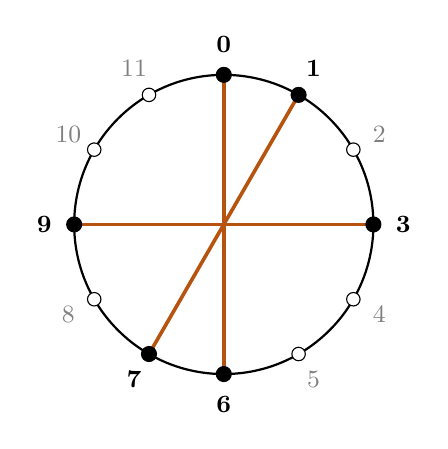
\begin{tikzpicture}[scale=1.9,every node/.style={font=\small}]
  \draw[thick] (0,0) circle (1);
  \foreach \a/\b in {0/6,1/7,3/9}{
    \draw[ctB,line width=1.3pt] ({90-30*\a}:1) -- ({90-30*\b}:1);
  }
  \foreach \k in {0,...,11}{
    \pgfmathtruncatemacro{\ina}{ ( \k==0 || \k==1 || \k==3 || \k==6 || \k==7 || \k==9 ) ? 1 : 0 }
    \ifnum\ina=1
      \filldraw[black] ({90-30*\k}:1) circle (0.05);
      \node at ({90-30*\k}:1.2) {\textbf{\k}};
    \else
      \draw[fill=white] ({90-30*\k}:1) circle (0.045);
      \node[gray] at ({90-30*\k}:1.2) {\k};
    \fi
  }
\end{tikzpicture}
\caption{\textbf{6-30} $=\{0,1,3,6,7,9\}$ on the pitch-class clock (filled nodes). It is the union of
the three central pairs $\{0,6\},\{1,7\},\{3,9\}$ (heavy tritone diameters), hence fixed by $T_6$ (a
$180^\circ$ rotation); with zero inversional symmetries it is \emph{not} inversionally symmetric. Choosing
three of the six tritone pairs, up to rotation/reflection, is the bracelet bijection of
\S\ref{sec:enum} (Figure~\ref{fig:bracelet}).}
\label{fig:clock}
\end{figure}

\begin{figure}[h]
\centering
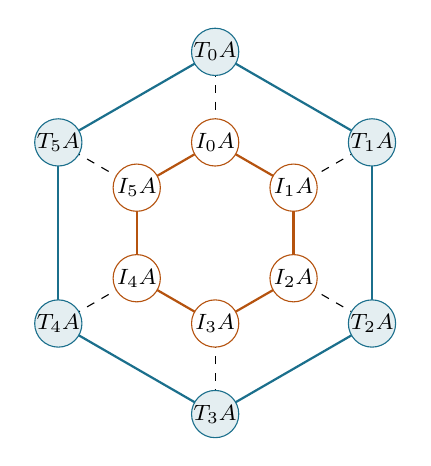
\begin{tikzpicture}[scale=1.0,every node/.style={font=\footnotesize},>={Stealth[length=2mm]}]
  \foreach \k in {0,...,5}{
    \coordinate (O\k) at ({90-60*\k}:2.3);
    \coordinate (I\k) at ({90-60*\k}:1.15);
  }
  \foreach \k in {0,...,5}{
    \pgfmathtruncatemacro{\next}{mod(\k+1,6)}
    \draw[ctA,->,thick] (O\k) -- (O\next);
    \draw[ctB,->,thick] (I\next) -- (I\k);
    \draw[dashed] (O\k) -- (I\k);
  }
  \foreach \k in {0,...,5}{
    \filldraw[fill=ctA!12,draw=ctA] (O\k) circle (0.30) node[black]{$T_{\k}A$};
    \filldraw[fill=white,draw=ctB] (I\k) circle (0.30) node[black]{$I_{\k}A$};
  }
\end{tikzpicture}
\caption{Cayley graph of the order-12 dual group $\Dgrp{6}$ acting simply transitively on the
$12$-element $T/I$-orbit of 6-30: the six transposition-forms $T_kA$ (outer, $T_kA=T_{k+6}A$ identified)
and the six inversion-forms $I_kA$ (inner). Solid arrows are an order-6 generator (orientation reverses
on the inner coset, as in any dihedral Cayley graph); dashed edges an order-2 generator. Regularity of
this action (\lean{Cgrp\_transitive} + semiregularity) is what makes the dual a group of order $12$.}
\label{fig:cayley}
\end{figure}

\section{How often does this happen?}\label{sec:enum}

\question{P\textsubscript{3}. Is $\Ztwelve$ special, or does a tritone-centered self-dual exist in every
universe? How many are there?}

For even $n$, count the set classes whose $T/I$-stabilizer is exactly the center $\{T_0,T_{n/2}\}$ (dual
$\cong\Dgrp{n/2}$, orbit $n$), by ranging over unions of the $n/2$ central pairs $\{x,x+n/2\}$
(\lean{sage/sixthirty.sage}):

\begin{table}[h]
\centering
\rowcolors{2}{ctA!7}{white}
\begin{tabular}{lrrrrrrrr}
\toprule
\rowcolor{ctA!22}
$n$    & 8 & 10 & \textbf{12} & 14 & 16 & 18 & 20 & 24\\
\midrule
count  & 0 & 0  & \textbf{1}  & 2  & 6  & 14 & 30 & 127\\
\bottomrule
\end{tabular}
\caption{Tritone-centered self-dual classes per universe $n$: none below $12$, unique at $12$ (the class
6-30).}
\label{tab:counts}
\end{table}

So $\Ztwelve$ is the smallest universe where the phenomenon exists, and there it is unique. The sequence
$1,2,6,14,30,62,127$ for $n=12,14,\dots,24$ is \textbf{OEIS A032239} (``number of identity (asymmetric)
bracelets of $m$ beads, $2$ colors'') at $m=n/2$. The bijection (Figure~\ref{fig:bracelet}): a
tritone-centered self-dual class is a choice of subset of the $n/2$ central pairs with trivial symmetry,
i.e.\ an asymmetric two-color bracelet on $n/2$ beads. There is no simple closed form (the tempting
$2^{m-5}-2$ fits $m=7..11$ then breaks at $m=12$: $\mathrm{A}032239(12)=127\ne126$); the enumeration is a
Burnside/P\'olya specialization. What is ours is the musical characterization, the bracelet bijection, and
the $\Ztwelve$-minimality of 6-30.

\begin{figure}[h]
\centering
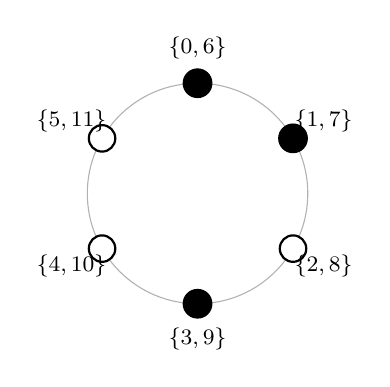
\begin{tikzpicture}[scale=1.4,every node/.style={font=\footnotesize}]
  \draw[gray!60] (0,0) circle (1);
  \foreach \i/\lab/\f in {0/{0,6}/1, 1/{1,7}/1, 2/{2,8}/0, 3/{3,9}/1, 4/{4,10}/0, 5/{5,11}/0}{
     \coordinate (b) at ({90-60*\i}:1);
     \ifnum\f=1 \filldraw[black] (b) circle (0.13);
     \else \draw[fill=white,thick] (b) circle (0.12); \fi
     \node at ({90-60*\i}:1.32) {$\{\lab\}$};
  }
\end{tikzpicture}
\caption{6-30 as a two-color bracelet on $m=6$ beads: bead $i$ is the central pair $\{i,i+6\}$, filled iff
in the set. The pattern (filled at $\{0,6\},\{1,7\},\{3,9\}$) has trivial rotation/reflection symmetry
--- an \emph{asymmetric} bracelet, the object counted by A032239; 6-30 is the unique such pattern at
$m=6$.}
\label{fig:bracelet}
\end{figure}

\section{What the dual is, musically}\label{sec:music}

\question{P\textsubscript{4}. The dual is an abstract group of order $12$. What is it \emph{for}?}

A simply transitive group action is exactly a \emph{Generalized Interval System} in Lewin's
sense~\cite[p.~157]{Lewin}: given any two elements there is a \emph{unique} operation carrying one to the
other. So the dual $\cong\Dgrp{6}$ is a GIS on the twelve forms of the Petrushka chord\,\audio{orbit_12.wav} ---
Figure~\ref{fig:cayley} is its map. Any form of the chord reaches any other by a unique dual move; the
twelve Petrushka colors become a single, navigable harmonic space, the symmetric-chord analogue of the
$P/L/R$ network for triads. Table~\ref{tab:family} places the result in its family.

\paragraph{Hear it.} Three sonifications accompany this note --- the Petrushka chord (two triads a
tritone apart), the $T_6$ invariance (6-30 and its tritone transpose share the same six pitch classes),
and a traversal of all twelve forms (the dual-group orbit, passing through the Petrushka chord at
$I_1$) --- as editable MIDI and rendered WAV:
\url{https://github.com/karlesmarin/music-math/tree/main/media}.

\begin{table}[h]
\centering\small
\setlength{\tabcolsep}{5pt}
\rowcolors{2}{ctA!7}{white}
\begin{tabular}{@{}lcccc@{}}
\toprule
\rowcolor{ctA!22}
Object & Stabilizer & Orbit & Dual & Order\\
\midrule
Triad (Crans--Fiore--Satyendra) & $\{T_0\}$ & $24$ & $\Dgrp{12}$ & $24$\\
Hexatonic cycle (Berry--Fiore) & $\{T_0,T_4,T_8\}$ (aug.) & $6$ & $S_3$ & $6$\\
\textbf{6-30 (this note)} & $\{T_0,T_6\}$ (tritone) & $12$ & $\Dgrp{6}$ & $12$\\
\bottomrule
\end{tabular}
\caption{Three instances of the same centralizer-duality machine, by the symmetry of the object.}
\label{tab:family}
\end{table}

\section{What is machine-checked}\label{sec:checked}

\question{P\textsubscript{5}. Can we trust all this?}

Everything stated about the duality engine and about 6-30 is checked by the Lean~4 kernel
(Tables~\ref{tab:lean}--\ref{tab:s30}); \lean{\#print axioms} returns exactly
\lean{[propext, Classical.choice, Quot.sound]} with no \lean{sorryAx} on every theorem. The enumeration
(Table~\ref{tab:counts}) and the named structure $\Dgrp{6}$ are additionally witnessed by re-runnable
Sage/GAP scripts (Table~\ref{tab:sage}).

\begin{table}[h]
\centering\small
\rowcolors{2}{ctA!7}{white}
\begin{tabular}{@{}l p{0.56\textwidth}@{}}
\toprule
\rowcolor{ctA!22}
\textbf{Theorem} & \textbf{Statement}\\
\midrule
\lean{centralizing\_fixedPoint\_eq\_one} & Wielandt regular case (centralizer of a transitive group is semiregular).\\
\lean{PLR\_le\_centralizer}              & $\langle P,L,R\rangle\le\mathrm{centralizer}(T/I)$.\\
\lean{card\_PLRgrp}                      & $\mathrm{Nat.card}\,\mathrm{PLRgrp}=24$.\\
\lean{centralizer\_eq\_PLR}             & $\mathrm{centralizer}(T/I)=\langle P,L,R\rangle$ (the CFS duality).\\
\bottomrule
\end{tabular}
\caption{The background duality engine in \lean{NeoRiemannian.lean} (namespace \lean{Duality}),
machine-checked (Brick 3).}
\label{tab:lean}
\end{table}

\begin{table}[h]
\centering\small
\rowcolors{2}{ctA!7}{white}
\begin{tabular}{@{}l p{0.60\textwidth}@{}}
\toprule
\rowcolor{ctA!22}
\textbf{Theorem} & \textbf{Statement}\\
\midrule
\lean{stab\_T}, \lean{stab\_I\_empty} & $\Stab_T(A)=\{0,6\}$; no inversional symmetry.\\
\lean{orbit\_card}                    & $T/I$-orbit of $A$ has $12$ elements.\\
\lean{Ker\_eq}                        & kernel of the $\Dgrp{12}$-action on the orbit $=Z=\{T_0,T_6\}$.\\
\lean{card\_TIgrpO}                   & image on the orbit $=\Dgrp{12}/Z$, order $12$.\\
\lean{card\_Cgrp}                     & the dual (centralizer on the orbit) has order $12$ (opposite regular rep).\\
\lean{Cgrp\_transitive}              & the dual is transitive, hence regular (simply transitive).\\
\lean{dihedral\_fingerprint}          & order $12$; $s$ of order $6$, $t^2=1$, $t\ne1$, $tst=s^{-1}$, $st\ne ts$.\\
\bottomrule
\end{tabular}
\caption{6-30's order-12 regular dihedral dual in \lean{SixThirty.lean}, machine-checked (Brick 19) ---
the first Lean proof of the structure of a symmetric chord's contextual dual.}
\label{tab:s30}
\end{table}

\begin{table}[h]
\centering\small
\rowcolors{2}{ctA!7}{white}
\begin{tabular}{@{}l p{0.58\textwidth}@{}}
\toprule
\rowcolor{ctA!22}
\textbf{Script} & \textbf{What it witnesses}\\
\midrule
\lean{centralizer\_witness.sage} & GAP: $PLR==\mathrm{centralizer}$ exactly; 6-30's 12-orbit dual $\cong\Dgrp{6}$.\\
\lean{sixthirty.sage}            & 6-30 detail (stab $\{T_0,T_6\}$, orbit 12, dual order 12) + counts per $n$.\\
\lean{duality\_sweep.sage}       & all $222$ $\Ztwelve$ classes: regular $\iff$ self-dual (0 exceptions).\\
\lean{sc630\_verify.sage}        & IV $=[2,2,4,2,2,3]$; stab $\{T_0,T_6\}$; not inversionally symmetric.\\
\bottomrule
\end{tabular}
\caption{Sage/GAP witnesses (Sage 10.8 + GAP), each re-runnable.}
\label{tab:sage}
\end{table}

\section{Novelty, scope, and open questions}\label{sec:novelty}

\paragraph{Contribution, stated plainly.} This is a formalization $+$ characterization note, not new
mathematics. The duality engine is the regular case of \textbf{Wielandt's centralizer theorem}
(\cite{DM} \S4.2 Thm 4.2A; \cite{Cam}); the contextual-group framework is
Fiore--Satyendra/Fiore--Noll~\cite{FS,FN11,FN25}. What is ours: (i) the reduced-duality characterization
with proof (Proposition~\ref{prop:dual}) and its tritone corollary (Lemma~\ref{lem:tritone}); (ii) the
6-30 instance with the \emph{first machine-checked} contextual dual of a symmetric chord
(Theorem~\ref{thm:sixthirty}, Brick 19); (iii) the enumeration and bracelet bijection. Mathlib has
\lean{DihedralGroup}, \lean{IsPretransitive} and Cayley's theorem, but no centralizer-of-regular-rep
result; our \lean{centralizing\_fixedPoint\_eq\_one} and the opposite-regular construction in
\lean{SixThirty.lean} fill that gap as first formalizations.

\paragraph{Relation to Berry--Fiore.} Berry--Fiore~\cite{BF} prove that the $PL$-group of a hexatonic
cycle is Lewin-dual to its $T/I$-stabilizer --- the same machine. The objects differ
(Table~\ref{tab:family}): theirs is the augmented-axis stabilizer $\{T_0,T_4,T_8\}$ with dual $S_3$ of
order $6$; ours is the tritone center $\{T_0,T_6\}$ with dual $\Dgrp{6}$ of order $12$. ``Tritone'',
``octatonic'', ``6-30'' do not appear in their paper.

\paragraph{Relation to Peck.} Peck~\cite{Peck} generalizes Lewin's commuting groups to semiregular and
diagonal actions with musical examples; we cite him for the machine. To our knowledge his treatment
includes neither our enumeration nor the specific order-12 instance --- verified against the abstract and
secondary literature only, as the \emph{JMT} body is paywalled; the published octatonic commuting groups
in this lineage are order $8$ ($\cong\Dgrp{4}$, \cite{FN11}), not order $12$. The order-12 instance sits
within Peck's ``diagonal cases'' remit and is hedged accordingly; the enumeration is the better-supported
novelty.

\paragraph{The lineage sidesteps the case (complementary, not missed).} Reads of \cite{FS,FN11,FN25}
confirm the tritone-central self-dual is unstated: each avoids the reduced-orbit regime differently
(ordered pc-segments $+$ a tritone condition; hypothesis-pruning of covers; ``no symmetries'' $+$ a
tritone condition that excludes $T_6$). Notably \cite{FN11} tabulates $\{0,1,4,6,7,10\}$ (``Major Triad
Tritone Mixture'') and studies its $2$-triad cover (dual order $2$) --- the \emph{same set class} as
6-30, never forming the order-12 dual of the hexachord-as-a-point. The proof-assistant literature has
only Prismriver~\cite{Prism} ($T/I$-only, no $PLR$/duality).

\question{P\textsubscript{6}. Where does the tritone lead next?}

\begin{itemize}\itemsep2pt
  \item \textbf{The general-$n$ family.} Proposition~\ref{prop:dual} is universe-independent; 6-30 is the
        minimal nontrivial instance of a family (dual $\cong\Dgrp{n/2}$ at universe $n$). A uniform
        statement and its Lean proof are open.
  \item \textbf{The named isomorphism.} We machine-check the dihedral \emph{fingerprint}
        (Table~\ref{tab:s30}); the named $\mathrm{dual}\cong\mathrm{DihedralGroup}\,6$ needs
        $\Dgrp{12}/Z\cong\Dgrp{6}$, currently a Mathlib gap (it is GAP-witnessed here).
  \item \textbf{Fourier.} $T_6$-symmetry is exactly even-frequency support of $\Ahat$ --- a magnitude
        fact; but self-duality needs phase information $|\Ahat|$ cannot see, the same blindness as the
        Z-relation. A phase-space account of self-duality is open.
  \item \textbf{Larger chords.} Seventh-chord and tetrachord analogues (cf.\ \cite{FN25}): is there a
        tritone-central self-dual among them?
\end{itemize}

The tritone that opens the Petrushka chord turns out to be the center of $\Dgrp{12}$, the obstruction in
Fourier space, and the seed of an order-12 self-duality --- one object seen from the keyboard, the
clock, the group, and now the Lean kernel. We have followed it as far as the machine can certify; it
points further.

\section*{Data and code availability}
The Lean sources (\lean{NeoRiemannian.lean}, \lean{SixThirty.lean}) and the Sage/GAP witness scripts of
Tables~\ref{tab:lean}--\ref{tab:sage} accompany this note; each Lean theorem is checkable by
\lean{\#print axioms} and each script is re-runnable.

\begin{thebibliography}{99}
\bibitem{CFS} A. S. Crans, T. M. Fiore, R. Satyendra, ``Musical actions of dihedral groups,''
  \emph{Amer. Math. Monthly} \textbf{116} (2009), no.~6, 479--495 (arXiv:0711.1873).
\bibitem{DM} J. D. Dixon, B. Mortimer, \emph{Permutation Groups}, Springer GTM 163, 1996
  (\S4.2, Theorem 4.2A).
\bibitem{Cam} P. J. Cameron, \emph{Permutation Groups}, London Math. Soc. Student Texts 45, CUP, 1999.
\bibitem{Lewin} D. Lewin, \emph{Generalized Musical Intervals and Transformations}, Yale Univ. Press,
  1987 (repr.\ Oxford Univ. Press, 2007); GIS $=$ simply transitive action, p.~157.
\bibitem{BF} C. Berry, T. M. Fiore, ``Hexatonic systems and dual groups in mathematical music theory,''
  \emph{Involve} \textbf{11} (2018), no.~2, 253--270 (arXiv:1602.02577).
\bibitem{Peck} R. W. Peck, ``Generalized commuting groups,'' \emph{J. Music Theory} \textbf{54} (2010),
  no.~2, 143--177. doi:10.1215/00222909-1214912.
\bibitem{FS} T. M. Fiore, R. Satyendra, ``Generalized contextual groups,'' \emph{Music Theory Online}
  \textbf{11}.3 (2005).
\bibitem{FN11} T. M. Fiore, T. Noll, ``Commuting groups and the topos of triads,'' in
  \emph{Mathematics and Computation in Music} (MCM 2011), LNCS \textbf{6726}, Springer, 2011, pp.~69--83
  (arXiv:1102.1496).
\bibitem{FN25} T. M. Fiore, T. Noll, E. Bonnell, H. Pyle, N. Rodriguez, M. Williams, S. Cannas,
  M. Andreatta, ``Transformations of triads and seventh chords: group extensions and duality,''
  arXiv:2507.20811 (2025).
\bibitem{Prism} L. Aniva, C. Wang, ``Prismriver: formalization of music theory and algorithmic
  composition in Lean~4,'' arXiv:2606.19936 (2026).
\bibitem{Berger} A. Berger, ``Problems of pitch organization in Stravinsky,'' \emph{Perspectives of New
  Music} \textbf{2} (1963), no.~1, 11--42.
\bibitem{Taruskin} R. Taruskin, \emph{Stravinsky and the Russian Traditions}, 2 vols., Univ. of
  California Press, 1996.
\bibitem{vandenToorn} P. C. van den Toorn, \emph{The Music of Igor Stravinsky}, Yale Univ. Press, 1983.
\bibitem{TymoczkoOct} D. Tymoczko, ``Stravinsky and the octatonic: a reconsideration,'' \emph{Music
  Theory Spectrum} \textbf{24} (2002), no.~1, 68--102.
\bibitem{Forte} A. Forte, \emph{The Structure of Atonal Music}, Yale Univ. Press, 1973.
\bibitem{OEIS} OEIS Foundation, sequence A032239, ``Number of identity bracelets of $n$ beads of 2
  colors.''
\end{thebibliography}

\end{document}
